\documentclass[12pt,a4paper,header]{abnt}

\usepackage[brazil]{babel}        
\usepackage[utf8]{inputenc} 

\usepackage{hyperref}
\usepackage{bookmark}
\usepackage{amsmath,amssymb,amsfonts,undertilde}
\usepackage{graphicx}
\usepackage{subfigure}
\usepackage{fancyhdr}



%%%%%%%%%%%%%%%%%%%%%%%%%%%
%Teoremas, definicoes, etc%
%%%%%%%%%%%%%%%%%%%%%%%%%%%

\newtheorem{thm}{Teorema}[section]
\newtheorem{cor}[thm]{Corolário}
\newtheorem{lem}[thm]{Lema}
\newtheorem{defi}[thm]{Definição}
\newtheorem{exe}[thm]{Exemplo}
\newtheorem{prop}[thm]{Proposição}

\renewcommand{\ABNTchapterfont}{\bfseries}
\renewcommand{\ABNTsectionfont}{\bfseries}

\fancypagestyle{logouff}{%
	\renewcommand{\headrulewidth}{0pt}
	\fancyhead{}
	\fancyhead[R]{
\includegraphics[width=0.7\textwidth]{logoUFF.pdf}}% Your logo/image
  	\setlength{\headheight}{30pt} 
  	\setlength{\headsep}{2cm}
}





\begin{document}

%%%%%%%%%%%%%%%%%%%%%%%%%%%%%%
%colocar aqui o nome do aluno%
%%%%%%%%%%%%%%%%%%%%%%%%%%%%%%
\autor{Leonardo Filgueira}


%%%%%%%%%%%%%%%%%%%%%%%%%%%%%%%%%%%%%
%colocar aqui o título da monografia%
%%%%%%%%%%%%%%%%%%%%%%%%%%%%%%%%%%%%%
\titulo{Sistemas de recomendação usando o software R}


%%%%%%%%%%%%%%%%%%%%%%%%%%%%%%%%%%%
%colocar aqui o nome do orientador%
%%%%%%%%%%%%%%%%%%%%%%%%%%%%%%%%%%%
\orientador{Luciane Ferreira Alcoforado}  


%%%%%%%%%%%%%%%%%%%%%%%%%%%%%%%%%%%%%%%%%%%%%%%%%%%
%colocar aqui o nome do co-orientador, caso exista%
%%%%%%%%%%%%%%%%%%%%%%%%%%%%%%%%%%%%%%%%%%%%%%%%%%%
\coorientador{Rodrigo Ribeiro}


%%%%%%%%%%%%%%%%%%%%%%%%%%%%%%%%%%%%%%%%%%%%%%%%%%%
%colocar aqui a data da apresentacao da monografia%
%%%%%%%%%%%%%%%%%%%%%%%%%%%%%%%%%%%%%%%%%%%%%%%%%%%
\data{30 de fevereiro de 2013}



%%%%%%%%%%%%%%%%%%%%%%%%%%%
%nao mexer até a linha 180%
%%%%%%%%%%%%%%%%%%%%%%%%%%%


\comentario{Monografia apresentada para obtenção do grau de Bacharel em Estatística pela Universidade Federal Fluminense.}

\instituicao{Departamento de Estatística \par Instituto de Matemática e Estatística \par Universidade Federal Fluminense}

\local{Niterói - RJ, Brasil}

\capa

\vspace{10cm}


%folha de rosto
%--------------

\begin{titlepage}

\thispagestyle{logouff}

\vspace{2cm}

\hspace{.2\textwidth} % posicionando a minipage
\begin{minipage}{.7\textwidth}

\begin{flushright}

{\large \bf \ABNTautordata} \\[3cm]

{\Large \bf \ABNTtitulodata}\\[3cm]

{\bf Trabalho de Conclusão de Curso}\\[1cm]

\end{flushright}

\begin{espacosimples}

\ABNTcomentariodata

\end{espacosimples}

\vspace{1cm}

\hfill Orientador: Prof. \ABNTorientadordata

\end{minipage}

\vspace{7cm}

\begin{center}

\ABNTlocaldata

\ABNTdatadata

\end{center}

\end{titlepage}


%ficha catalografica
%-------------------
\newpage
\null
\vfill

%\begin{left}
\fbox{
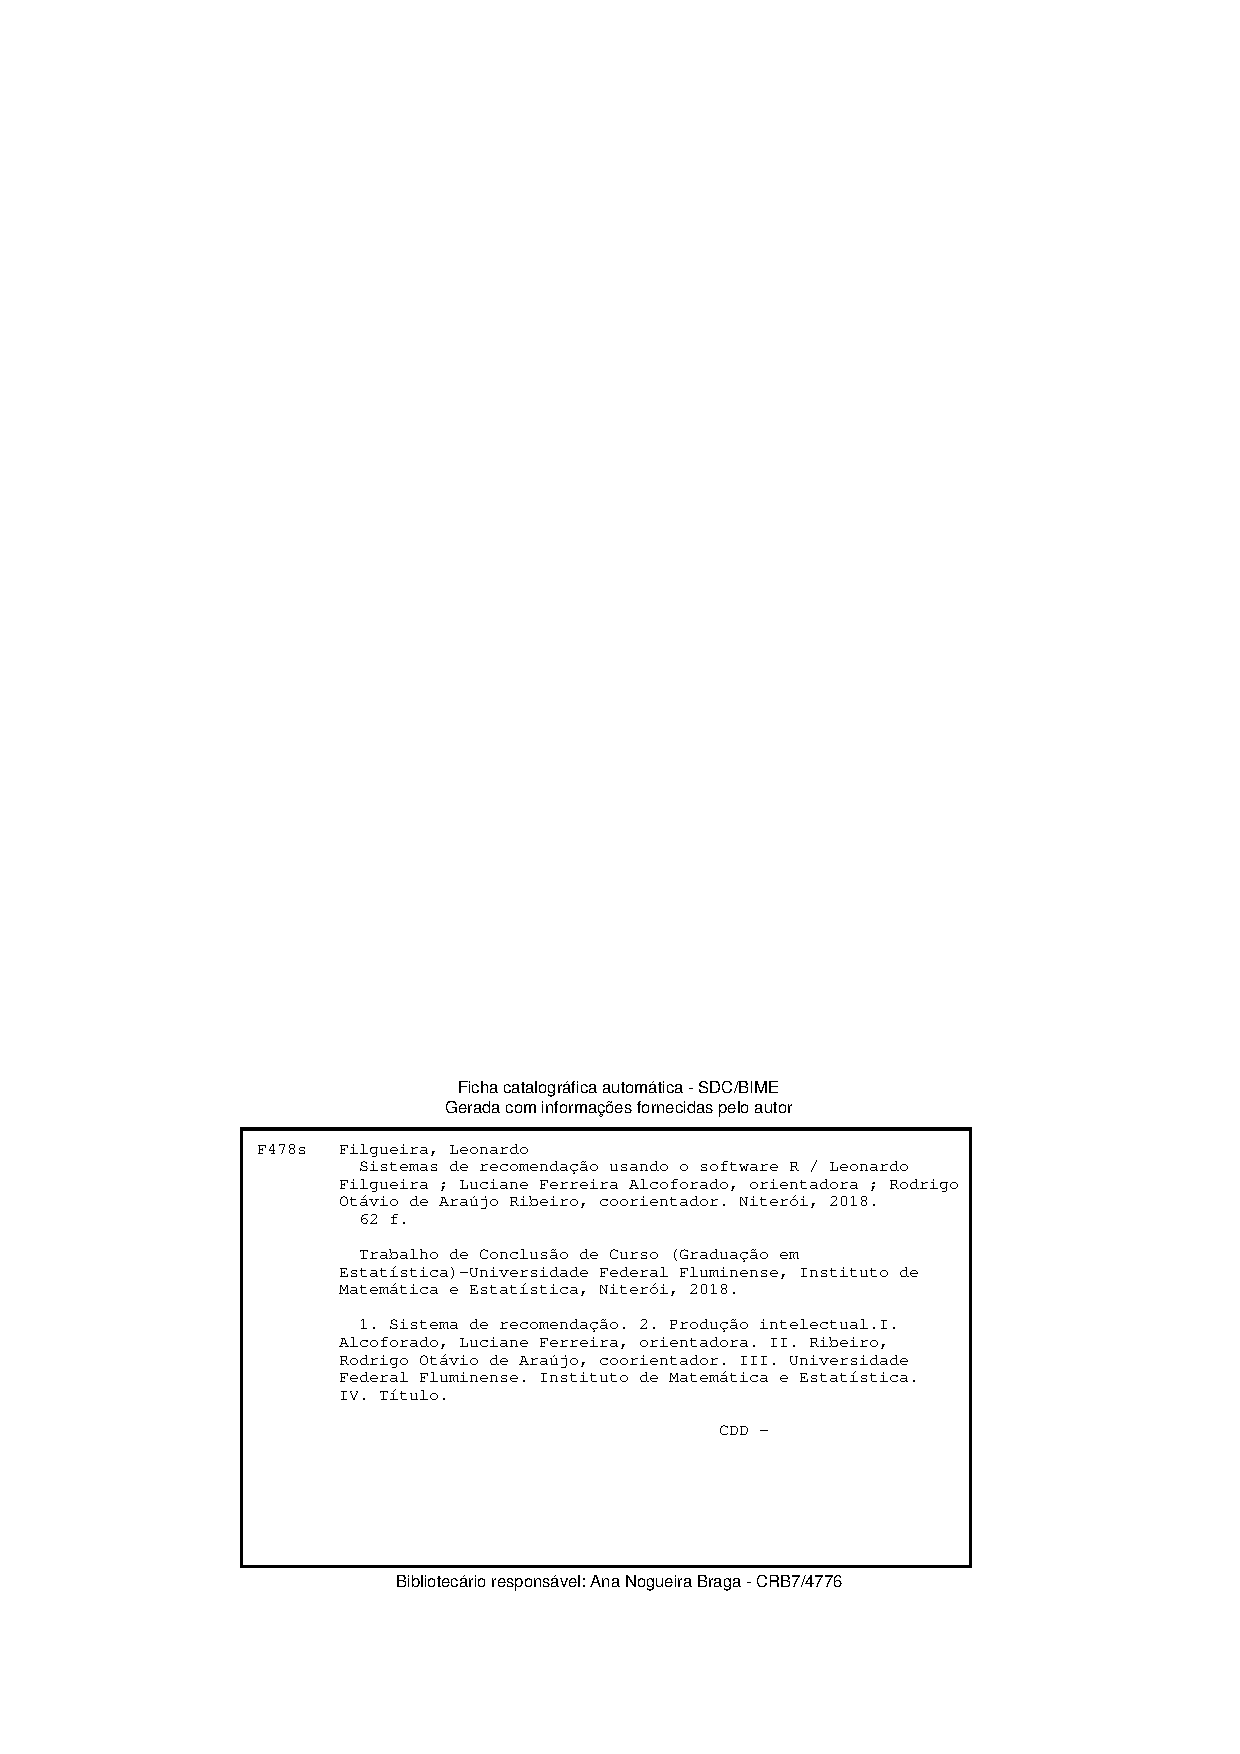
\includegraphics[scale=1]{ficha_catalografica.pdf}
}
%\end{center}
\vspace{1cm}

%folha de aprovacao com as assinaturas - Editar os membros da banca
%------------------------------------------------------------------
\begin{folhadeaprovacao}

\thispagestyle{logouff}

\hspace{.2\textwidth} % posicionando a minipage
\begin{minipage}{.7\textwidth}

\begin{flushright}

{\large \bf \ABNTautordata}\\[1cm]

{\large \bf \ABNTtitulodata}\\[1cm]

\end{flushright}

Monografia de Projeto Final de Graduação sob o título \textit{``\ABNTtitulodata''},
defendida por \ABNTautordata~e aprovada em \ABNTdatadata, na cidade de Niterói,
no Estado do Rio de Janeiro, pela banca examinadora constituída pelos
professores:

\begin{flushright}

\begin{espacosimples}

%assinatura




%%%%%%%%%%%%%%%%%%%%%%%%%%%%%%%%%%%%%%%%%
%Preencher os dados dos membros da banca%
%%%%%%%%%%%%%%%%%%%%%%%%%%%%%%%%%%%%%%%%%

\vspace{2cm}
\noindent\rule{8cm}{0.4pt}\\
{\bf Profa. Dra. Luciane Ferreira Alcoforado}\\
Departamento de Estatística -- UFF\\


\vspace{2cm}
\noindent\rule{8cm}{0.4pt}\\
{\bf Prof. Dr. Nome do 1o membro da banca}\\
Instituicao do 1o membro da banca\\


\vspace{2cm}
\noindent\rule{8cm}{0.4pt}\\
{\bf Profa. Me. Nome do 2o membro da banca}\\
Instituicao do 2o membro da banca\\

\end{espacosimples}

\end{flushright}

\vspace{2cm}
\hfill Niterói, \ABNTdatadata

\end{minipage}


%\vfill \hfill Niterói, \ABNTdatadata \hspace{1cm} 


\end{folhadeaprovacao}




%%%%%%%%%%%%%%%%%%%%%%%%%%%%%%%%%%%%%%%
%escreva aqui o resumo do seu trabalho%
%%%%%%%%%%%%%%%%%%%%%%%%%%%%%%%%%%%%%%%
\begin{resumo}
Aqui entra o resumo da monografia.

\vspace{1cm}
\noindent Palavras-chaves: 
%Aqui entram as palavras chaves.


\end{resumo}



%%%%%%%%%%%%%%%%%%%%%%%%%%%%%%%%
%escreva aqui a sua dedicatória% (opcional)
%%%%%%%%%%%%%%%%%%%%%%%%%%%%%%%%
\chapter*{Dedicatória}
Aqui entra a sua dedicatória. 



%%%%%%%%%%%%%%%%%%%%%%%%%%%%%%%%%%
%escreva aqui seus agradecimentos% (opcional)
%%%%%%%%%%%%%%%%%%%%%%%%%%%%%%%%%%
\chapter*{Agradecimentos}
Aqui entram os agradecimentos. 



\tableofcontents{}
\listoffigures
\listoftables



\chapter{Introdução} \label{cap:introducao}

A partir do aumento de informação disponível com a popularização da Internet e com a possibilidade de armazenar essas informações surge o desafio de lidar com este grande conjunto de dados\cite{isinkaye2015recommendation}. Este aumento de informações desafia o site, como lojas on-line, que recebem todas as informações dos usuários que visitam o endereço, mas também pode se tornar um problema para o usuário que, diante da grande quantidade de produtos disponíveis para compra, pode levar muito tempo para achar o produto desejado\cite{mild2002collaborative}.

Sistemas de recomendação são técnicas de \textit{machine learning} que filtram um grande conjunto de dados, tendo como base informações dos usuários\cite{takahashi2015estudo}. A partir dessas técnicas são previstas as notas que os usuários dariam a determinados itens, que podem ser dos mais variados tipos, e, para um indivíduo, recomenda-se o(s) item(ns) que obtiveram uma nota prevista maior\cite{shapira2011recommender}. Os sistemas de recomendação têm como objetivo recomendar itens que interessariam aos usuários\cite{melville2011recommender}, beneficiando o usuário e a loja, pois eles aumentam o desempenho da loja, fazendo-a vender uma quantidade maior de produtos, e também facilitam a procura do usuário fazendo-o achar produto(s) desejados em menos tempo\cite{isinkaye2015recommendation}. 

É facilmente perceptível no cotidiano o uso de sistemas de recomendação em ambientes on-line. Ao usar a \textit{Netflix}, sugestões para o usuário são oferecidas, baseadas nas atrações já assistidas e/ou avaliadas. Sites de compras como a \textit{Amazon} também oferecem sugestões de produtos ao usuário baseado em visitas à página dos produtos ou no comportamento de outros usuários que compraram um mesmo produto. Também em redes sociais, como no \textit{YouTube}, são sugeridos vídeos baseados no histórico do internauta e nas suas avaliações, ou então no \textit{Facebook}, que recomenda lista de pessoas que o usuário pode conhecer\cite{gorakala2015building}.

Em geral, sistemas de recomendação utilizam como informação a avaliação (\textit{rating}) dada pelos usuários aos itens, podendo a avaliação estar expressa de diferentes maneiras\cite{shapira2011recommender}:

\begin{itemize}

\item Avaliações numéricas: O usuário avalia um item numa escala numérica, como no site da \textit{Amazon}, onde o usuário dá uma nota de até 5 estrelas.

\item Avaliações qualitativas: A avaliação é dada por frases definidas, como: "Concordo totalmente", "Concordo parcialmente", ...

\item Avaliações binárias: O usuário seleciona se gostou ou não gostou do item, como a \textit{Netflix}, atualmente, recebe as avaliações.

\item Avaliação unária: A indicação se refere a se o usuário visualizou, comprou ou então avaliou o item positivamente.

\end{itemize}

Os algoritmos de recomendação utilizam uma matriz, chamada de matriz de avaliações (\textit{ratings matrix}), usualmente representada desta forma:

\begin{table}[!h]
\centering
\caption{Típica matriz de avaliações}
\label{rating_matrix}
\begin{tabular}{c|c|c|c|c}
\hline \\
            & Item 1      & Item 2      & $\cdots$ & Item m      \\
Usuário 1   & $r_{(1, 1)}$ &             & $\cdots$  &             \\
Usuário 2   &  & $r_{(2, 2)}$ & $\cdots$ & $r_{(2, m)}$ \\
$\vdots$       &    $\vdots$  & $\vdots$       &  $\ddots$ & $\vdots$ \\
Usuário $n$ & $r_{(n, 1)}$ &             & $\cdots$ & $r_{(n, m)}$ \\
\hline
\end{tabular}
\end{table}

Onde $r_{(i, j)}$ é a avaliação (\textit{rating}) do usuário $i$ dado ao item $j$. Em geral, os usuários não tiveram contato com todos os itens, então os itens não recebem avaliações de todos os usuários, produzindo então uma matriz esparsa (com grande quantidade de valores faltantes). Os algoritmos buscam, então, preencher a matriz de avaliações com previsões para os valores faltantes.

\section{Técnicas de recomendação}

Existem diferentes categorias de sistemas de recomendação, que podem ser classificados em: Filtragem baseada em conteúdo (\textit{Content-based filtering}), filtragem colaborativa (\textit{Collaborative filtering}) e sistemas de recomendação híbridos (\textit{Hybrid Recommender Systems})\cite{melville2011recommender}.

\subsection{Filtragem baseada em conteúdo}

A ideia por trás dos sistemas nesta categoria é recomendar itens similares aos que o usuário gostou no passado\cite{gorakala2015building}. Para isto é necessário quantificar a similaridade entre itens, utilizando informações das características de um produto\cite{shapira2011recommender}. Considerando filmes como itens, se um usuário avaliou positivamente filmes do gênero de ação, então o sistema recomendará a este usuário filmes de ação.

\subsection{Filtragem colaborativa}

\subsection{Sistemas de recomendação híbridos}


\chapter{Objetivos}

Este trabalho tem os seguintes objetivos:

\section{Objetivo geral}

\begin{itemize}

\item{Apresentar técnicas de sistemas de recomendação, executar algumas destas técnicas e avaliá-las.}

\end{itemize}

\section{Objetivos específicos}


\chapter{Materiais e Métodos}

Apresente aqui os materiais e métodos usados na monografia. 

Este capítulo pode ser modificado de acordo com o interesse do aluno e do orientador, dependendo do trabalho desenvolvido. Crie tantas seções quantas forem necessárias; a revisão bibliográfica pode também ser incluída aqui.


\section{Algumas Dicas}

Separe em seções para organizar melhor seu texto. Use os comandos \verb|\section| e \verb|\subsection| para isso. 

Sempre que preciso faça as referências usando o comando \verb|\cite|, como por exemplo, ``para mais informações sobre esse assunto veja o livro de Larson.''

Use os comandos a seguir para apresentar teoremas, definições, proposições, exemplos, etc. Dessa forma a numeração é feita de forma automática. 

{\defi
Abra e feche as chaves e dentro delas coloque o comando \verb|\defi| seguido da definição. 
}

{\thm
Abra e feche as chaves e dentro delas coloque o comando \verb|\thm| seguido do enunciado do teorema. 
}

{\prop
Abra e feche as chaves e dentro delas coloque o comando \verb|\prop| seguido do enunciado da proposição.
}


{\exe
Abra e feche as chaves e dentro delas coloque o comando \verb|\exe| seguido do exemplo.
}




\chapter{Análise dos Resultados}


Neste capítulo deve-se apresentar os resultados, podendo comentá-los e discuti-los, comparando-os com resultados da bibliografia já existente. Use seções, se apropriado.

Para que as tabelas e figuras sejam incluídas corretamente nas listas de tabelas e figuras use os comandos 
\verb|\begin{table}...\end{table}| e \verb|\begin{figure}...\end{figure}|. Veja como nos exemplos a seguir.

Primeiro o exemplo de uma tabela. 

\begin{table}[h!]
\centering
\caption{Tabela exemplo} \label{fig:exemplo}
\begin{tabular}{cc}
\hline
Ano & Produção (1.000t)\\
\hline
1996 & 2.536\\
1997 & 2.666\\
1998 & 3.750\\
1999 & 2.007\\
2000 & 2.080\\
\hline
\end{tabular}
\end{table}

Agora veja como incluir figuras.

\begin{figure}[h!]
\centering

\includegraphics[width=0.5\linewidth]{logoUFF.pdf}
\caption{Figura exemplo} \label{tab:exemplo}
\end{figure}

Use o comando \verb|ref| para fazer referências das tabelas e figuras ao longo do texto. Por exemplo, podemos nos referencias à Figura \ref{fig:exemplo} ou à Tabela \ref{tab:exemplo}. 

O mesmo comando \verb|ref| pode ser usado para fazer referência à capítulos, seções, equações, etc. Basta que tenha sido definido um \verb|label| para cada um deles. Por exemplo, se quisermos fazer referência ao número do capítulo Introdução basta digitar \verb|\ref{cap:introducao}|, veja como: ``... como comentado no Capítulo \ref{cap:introducao}, na introdução deste trabalho''. 




\chapter{Conclusão}

Para finalizar seu trabalho faça o capítulo de conclusão. Neste capítulo deve ser feito um breve resumo de tudo que foi feito e as principais conclusões obtidas.



%A bibliografia é feita automaticamente com o comando abaixo
%No arquivo referencias.bib devem ser incluídos todos os textos referenciados nesse trabalho.
\bibliographystyle{abnt-num} %abnt-num ou abnt-alf
\bibliography{referencias}


%Os anexos devem ser intorduzidos ao final do trabalho, depois das referências
\anexo



\chapter{Título do primeiro anexo}

Caso você ache interessante, adicione anexos ao trabalho. Estes devem vir depois das referências bibliográficas. 



\chapter{Título do segundo anexo}

Dessa forma você pode incluir quantos anexos quiser. 




\end{document}
